\documentclass{beamer}
\usepackage[utf8]{inputenc}
\usepackage[final]{pdfpages}

\usetheme{Goettingen}%Warsaw}
\usecolortheme{lily}
\setbeamertemplate{footline}[page number]
\title[A Case for Scaling Applications to Many-core with OS Clustering ]{A Case for Scaling Applications to Many-core with OS Clustering}
\author{
(reviewed by Oleg Iegorov and Jander Nascimento)}
\institute{University Joseph Fourier}
\date{\today}
\begin{document}

\begin{frame}
\titlepage
\end{frame}

%\AtBeginSubsection[]
{
  \begin{frame}<beamer>
    \frametitle{Roadmap}
    \tableofcontents%[currentsection,currentsubsection]
  \end{frame}
}

%this is filled up with some sample code (we can remove it anytime)

\section{Super process}

	\begin{frame}{Transferring process}

	\begin{itemize}
	\item Create local process
	\item Saves the state of the process
	\item Request target VM to create a process
	\item Target VM create its own process
	\item Target VM restores the state
	\end{itemize}
	
	\end{frame}	
	
	\begin{frame}{Performance techniques}

	\begin{itemize}
	\item Only certain levels of the page tables are shared
	\item Use domains to address page faults
	\item Avoid conflicting by enforcing update memory state
	\end{itemize}
	
	\end{frame}
	
	\begin{frame}{Shared Data Segment}
	
	\begin{itemize}	
		\item Not common for multiprocess application
		\item Very common for multi-threaded
	\end{itemize}	
		
	\end{frame}

	\begin{frame}{Cerberus arch}

		\begin{figure} [H]
			\centering
			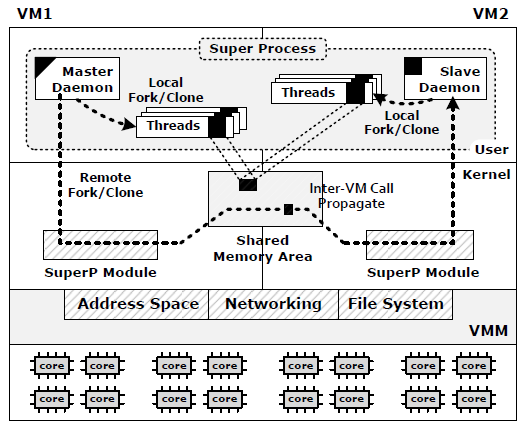
\includegraphics[scale=0.40]{img/cerberus-architecture}
		\end{figure}	

	\end{frame}

	\begin{frame}{Syscall virtualization}
	
		\begin{figure} [H]
			\centering
			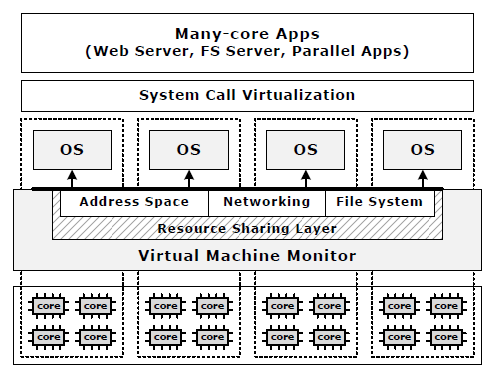
\includegraphics[scale=0.40]{img/syscall-virtualization}
		\end{figure}	

	\end{frame}
	
	\begin{frame}{Fork and Clone}
	
		\begin{figure} [H]
			\centering
			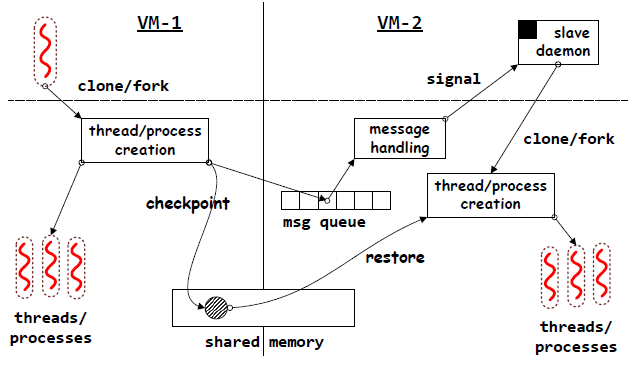
\includegraphics[scale=0.40]{img/cerberus-fork-clone}
		\end{figure}	
	
	\end{frame}

\section{Sharing file}
	
	\begin{frame}{Common approach}	
	
		Use existent network file systems:
		\begin{itemize}
		\item NFS
		\end{itemize}
		
		Issues?
		\begin{itemize}
		\item Centralized
		\item Rather slow
		\end{itemize}		

		\begin{alertblock}{}
			Solution?
		\end{alertblock}

	\end{frame}	
	
	\begin{frame}{Sharing file}	
	
		\begin{block}{Question}
			How share data files?
		\end{block}
		
		The answer might be:		
		\begin{itemize}
		\item Hybrid solution: local and remote file access.
		\item Basic security scheme: public or private file.
		\end{itemize}

	\end{frame}

	\begin{frame}{CFS arch}

		\begin{figure} [H]
			\centering
			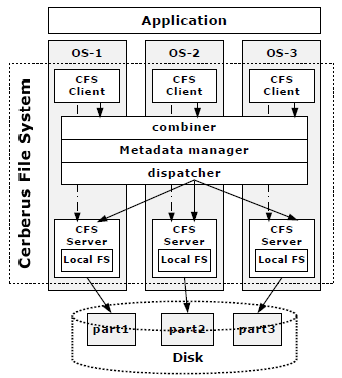
\includegraphics[scale=0.40]{img/cerberus-cfs}
		\end{figure}	

	\end{frame}

\section{The prototype}

	\begin{frame}{Prototype}

	Technical stuff:
	\begin{itemize}
	\item based on Xen
	\item Uses compare and swap to look for gaps
	\item using shadow mode page table
	\item re-implement a subset of POSIX calls
	\item Using P2M
	\end{itemize}
	
	\end{frame}

\section{Evaluation}

\section{Conclusion}



\end{document}
